%=====================================================================
%            CHAPITRE 4 : RÉALISATION
%=====================================================================

\chapter{Réalisation}

%---------------------------------------------------------------------
\section{Introduction}
%---------------------------------------------------------------------

Ce chapitre présente la réalisation technique de l'application RouteChain. Nous décrirons l'environnement de développement utilisé, puis nous détaillerons les technologies employées pour chaque couche de l'application avec leurs justifications de choix. Enfin, nous présenterons les principales interfaces utilisateur développées.

%---------------------------------------------------------------------
\section{Environnement de Développement}
%---------------------------------------------------------------------

\subsection{Outils de Développement}

\begin{table}[H]
\centering
\caption{Outils de développement utilisés}
\begin{tabular}{|l|l|}
\hline
\textbf{Catégorie} & \textbf{Outil} \\
\hline
IDE & Visual Studio Code \\
Contrôle de version & Git \\
Gestionnaire de paquets Python & pip \\
Gestionnaire de paquets Node & npm \\
Navigateur de test & Google Chrome / Safari \\
Client API & Postman \\
\hline
\end{tabular}
\end{table}

\subsection{Structure du Projet}

Le projet est organisé en trois répertoires principaux : \texttt{backend/} pour l'API Python, \texttt{frontend/} pour l'interface React, et \texttt{blockchain/} pour les smart contracts Solidity.

%---------------------------------------------------------------------
\section{Technologies Backend}
%---------------------------------------------------------------------

\subsection{Python}
\textbf{Définition :} Python est un langage de programmation interprété, multi-paradigme et dynamiquement typé. Reconnu pour sa syntaxe claire et sa lisibilité, il est largement utilisé dans le développement web, la science des données et l'automatisation.

\begin{figure}[H]
\centering
\includegraphics[width=2.5cm]{logos/python.png}
\caption{Logo Python}
\end{figure}

\textbf{Justification du choix :}
\begin{itemize}
    \item Écosystème riche pour le développement web (FastAPI, Flask, Django)
    \item Excellentes bibliothèques pour l'optimisation (OR-Tools, SciPy)
    \item Intégration native avec Web3.py pour la blockchain
    \item Syntaxe expressive accélérant le développement
\end{itemize}

\subsection{FastAPI}
\textbf{Définition :} FastAPI est un framework web Python moderne et performant pour la création d'APIs RESTful. Basé sur les standards OpenAPI et JSON Schema, il offre une validation automatique des données et une documentation interactive générée automatiquement.

\begin{figure}[H]
\centering
\includegraphics[width=3cm]{logos/fastapi.png}
\caption{Logo FastAPI}
\end{figure}


\textbf{Justification du choix :}
\begin{itemize}
    \item Performances exceptionnelles comparables à Node.js et Go
    \item Validation automatique via les type hints Python
    \item Documentation Swagger/OpenAPI générée automatiquement
    \item Support natif de l'asynchrone (async/await)
    \item Intégration facile avec Pydantic pour la sérialisation
\end{itemize}

\subsection{MongoDB}
\textbf{Définition :} MongoDB est une base de données NoSQL orientée documents. Elle stocke les données sous forme de documents JSON flexibles (BSON), permettant une modélisation naturelle des données et une évolutivité horizontale.

\begin{figure}[H]
\centering
\includegraphics[width=3.5cm]{logos/mongodb.png}
\caption{Logo MongoDB}
\end{figure}


\textbf{Justification du choix :}
\begin{itemize}
    \item Schéma flexible adapté aux données de tournées variables
    \item Stockage natif des objets imbriqués (points de livraison)
    \item MongoDB Atlas offre un hébergement cloud gratuit
    \item Driver Motor asynchrone pour de meilleures performances
    \item Requêtes géospatiales natives pour les coordonnées GPS
\end{itemize}

\subsection{Google OR-Tools}
\textbf{Définition :} Google OR-Tools est une suite open-source d'outils pour l'optimisation combinatoire. Elle inclut des solveurs pour les problèmes de programmation linéaire, de routage de véhicules (VRP), et de satisfaction de contraintes.

\begin{figure}[H]
\centering
\includegraphics[width=3cm]{logos/or_tools.png}
\caption{Logo Google OR-Tools}
\end{figure}

\newpage

\textbf{Justification du choix :}
\begin{itemize}
    \item Solveur VRP de référence développé par Google
    \item Multiples stratégies d'optimisation configurables
    \item Support des contraintes complexes (capacité, fenêtres temporelles)
    \item Performances optimisées pour les problèmes à grande échelle
    \item Documentation complète et exemples Python
\end{itemize}

%---------------------------------------------------------------------
\section{Technologies Frontend}
%---------------------------------------------------------------------

\subsection{React}
\textbf{Définition :} React est une bibliothèque JavaScript développée par Meta pour la construction d'interfaces utilisateur. Basée sur le concept de composants réutilisables et le DOM virtuel, elle permet un développement efficace d'applications web interactives.

\begin{figure}[H]
\centering
\includegraphics[width=2.5cm]{logos/react.png}
\caption{Logo React}
\end{figure}


\textbf{Justification du choix :}
\begin{itemize}
    \item Architecture composants favorisant la réutilisabilité
    \item Virtual DOM assurant des performances optimales
    \item Écosystème mature avec nombreuses bibliothèques
    \item Large communauté et documentation abondante
    \item Hooks simplifiant la gestion de l'état
\end{itemize}

\subsection{Vite}
\textbf{Définition :} Vite est un outil de build nouvelle génération pour le développement web. Il exploite les modules ES natifs du navigateur pour offrir un démarrage instantané et un Hot Module Replacement (HMR) ultra-rapide.

\begin{figure}[H]
\centering
\includegraphics[width=2.5cm]{logos/vite.png}
\caption{Logo Vite}
\end{figure}


\textbf{Justification du choix :}
\begin{itemize}
    \item Démarrage du serveur de développement instantané
    \item Hot Module Replacement en moins de 50ms
    \item Build de production optimisé avec Rollup
    \item Configuration minimale requise
    \item Support natif de TypeScript et JSX
\end{itemize}

\subsection{Tailwind CSS}
\textbf{Définition :} Tailwind CSS est un framework CSS utilitaire qui fournit des classes de bas niveau pour construire des designs personnalisés directement dans le HTML. Il privilégie la composition plutôt que l'abstraction.

\begin{figure}[H]
\centering
\includegraphics[width=3cm]{logos/tailwind.png}
\caption{Logo Tailwind CSS}
\end{figure}


\textbf{Justification du choix :}
\begin{itemize}
    \item Développement rapide sans quitter le HTML/JSX
    \item Design system cohérent avec configuration centralisée
    \item Purge automatique du CSS non utilisé en production
    \item Responsive design intégré avec préfixes (sm:, md:, lg:)
    \item Personnalisation complète via tailwind.config.js
\end{itemize}

\subsection{Leaflet}
\textbf{Définition :} Leaflet est une bibliothèque JavaScript open-source pour les cartes interactives. Légère et modulaire, elle offre toutes les fonctionnalités de cartographie nécessaires tout en restant simple à utiliser.


\begin{figure}[H]
\centering
\includegraphics[width=3cm]{logos/leaflet.png}
\caption{Logo Leaflet}
\end{figure}


\textbf{Justification du choix :}
\begin{itemize}
    \item Bibliothèque légère (42KB gzippée)
    \item Compatible avec OpenStreetMap (gratuit)
    \item API simple et bien documentée
    \item Support des marqueurs, polylignes et popups personnalisés
    \item Plugin react-leaflet pour intégration React
\end{itemize}

\subsection{Axios}
\textbf{Définition :} Axios est un client HTTP basé sur les promesses pour le navigateur et Node.js. Il simplifie les requêtes AJAX avec une API intuitive et des fonctionnalités avancées comme les intercepteurs.

\begin{figure}[H]
\centering
\includegraphics[width=2.5cm]{logos/axios.png}
\caption{Logo Axios}
\end{figure}


\textbf{Justification du choix :}
\begin{itemize}
    \item Syntaxe simple basée sur les promesses/async-await
    \item Intercepteurs pour gérer l'authentification JWT
    \item Transformation automatique des données JSON
    \item Gestion des erreurs centralisée
    \item Annulation des requêtes avec AbortController
\end{itemize}

%---------------------------------------------------------------------
\section{Technologies Blockchain}
%---------------------------------------------------------------------

\subsection{Ganache}
\textbf{Définition :} Ganache est un simulateur de blockchain Ethereum personnel pour le développement. Il permet de déployer des contrats, développer des DApps et exécuter des tests dans un environnement local contrôlé.

\begin{figure}[H]
\centering
\includegraphics[width=3cm]{logos/ganache.png}
\caption{Logo Ganache}
\end{figure}


\textbf{Justification du choix :}
\begin{itemize}
    \item Blockchain locale instantanée sans synchronisation
    \item Interface graphique pour visualiser les transactions
    \item Comptes pré-financés pour les tests
    \item Mining instantané des blocs
    \item Persistance des données via workspaces
\end{itemize}

%---------------------------------------------------------------------
\section{Présentation des Interfaces Utilisateur}
%---------------------------------------------------------------------

\subsection{Écrans d'Authentification}

L'application RouteChain propose un système d'authentification sécurisé comprenant une page de connexion et une page d'inscription. La page de connexion présente une interface épurée et moderne, permettant aux chauffeurs de s'authentifier avec leur email et mot de passe. Le design utilise une palette de couleurs professionnelle dominée par le bleu, avec des champs de saisie clairement identifiés et un bouton de connexion bien visible. Un lien vers la page d'inscription est proposé pour les nouveaux utilisateurs.

\begin{figure}[H]
\centering
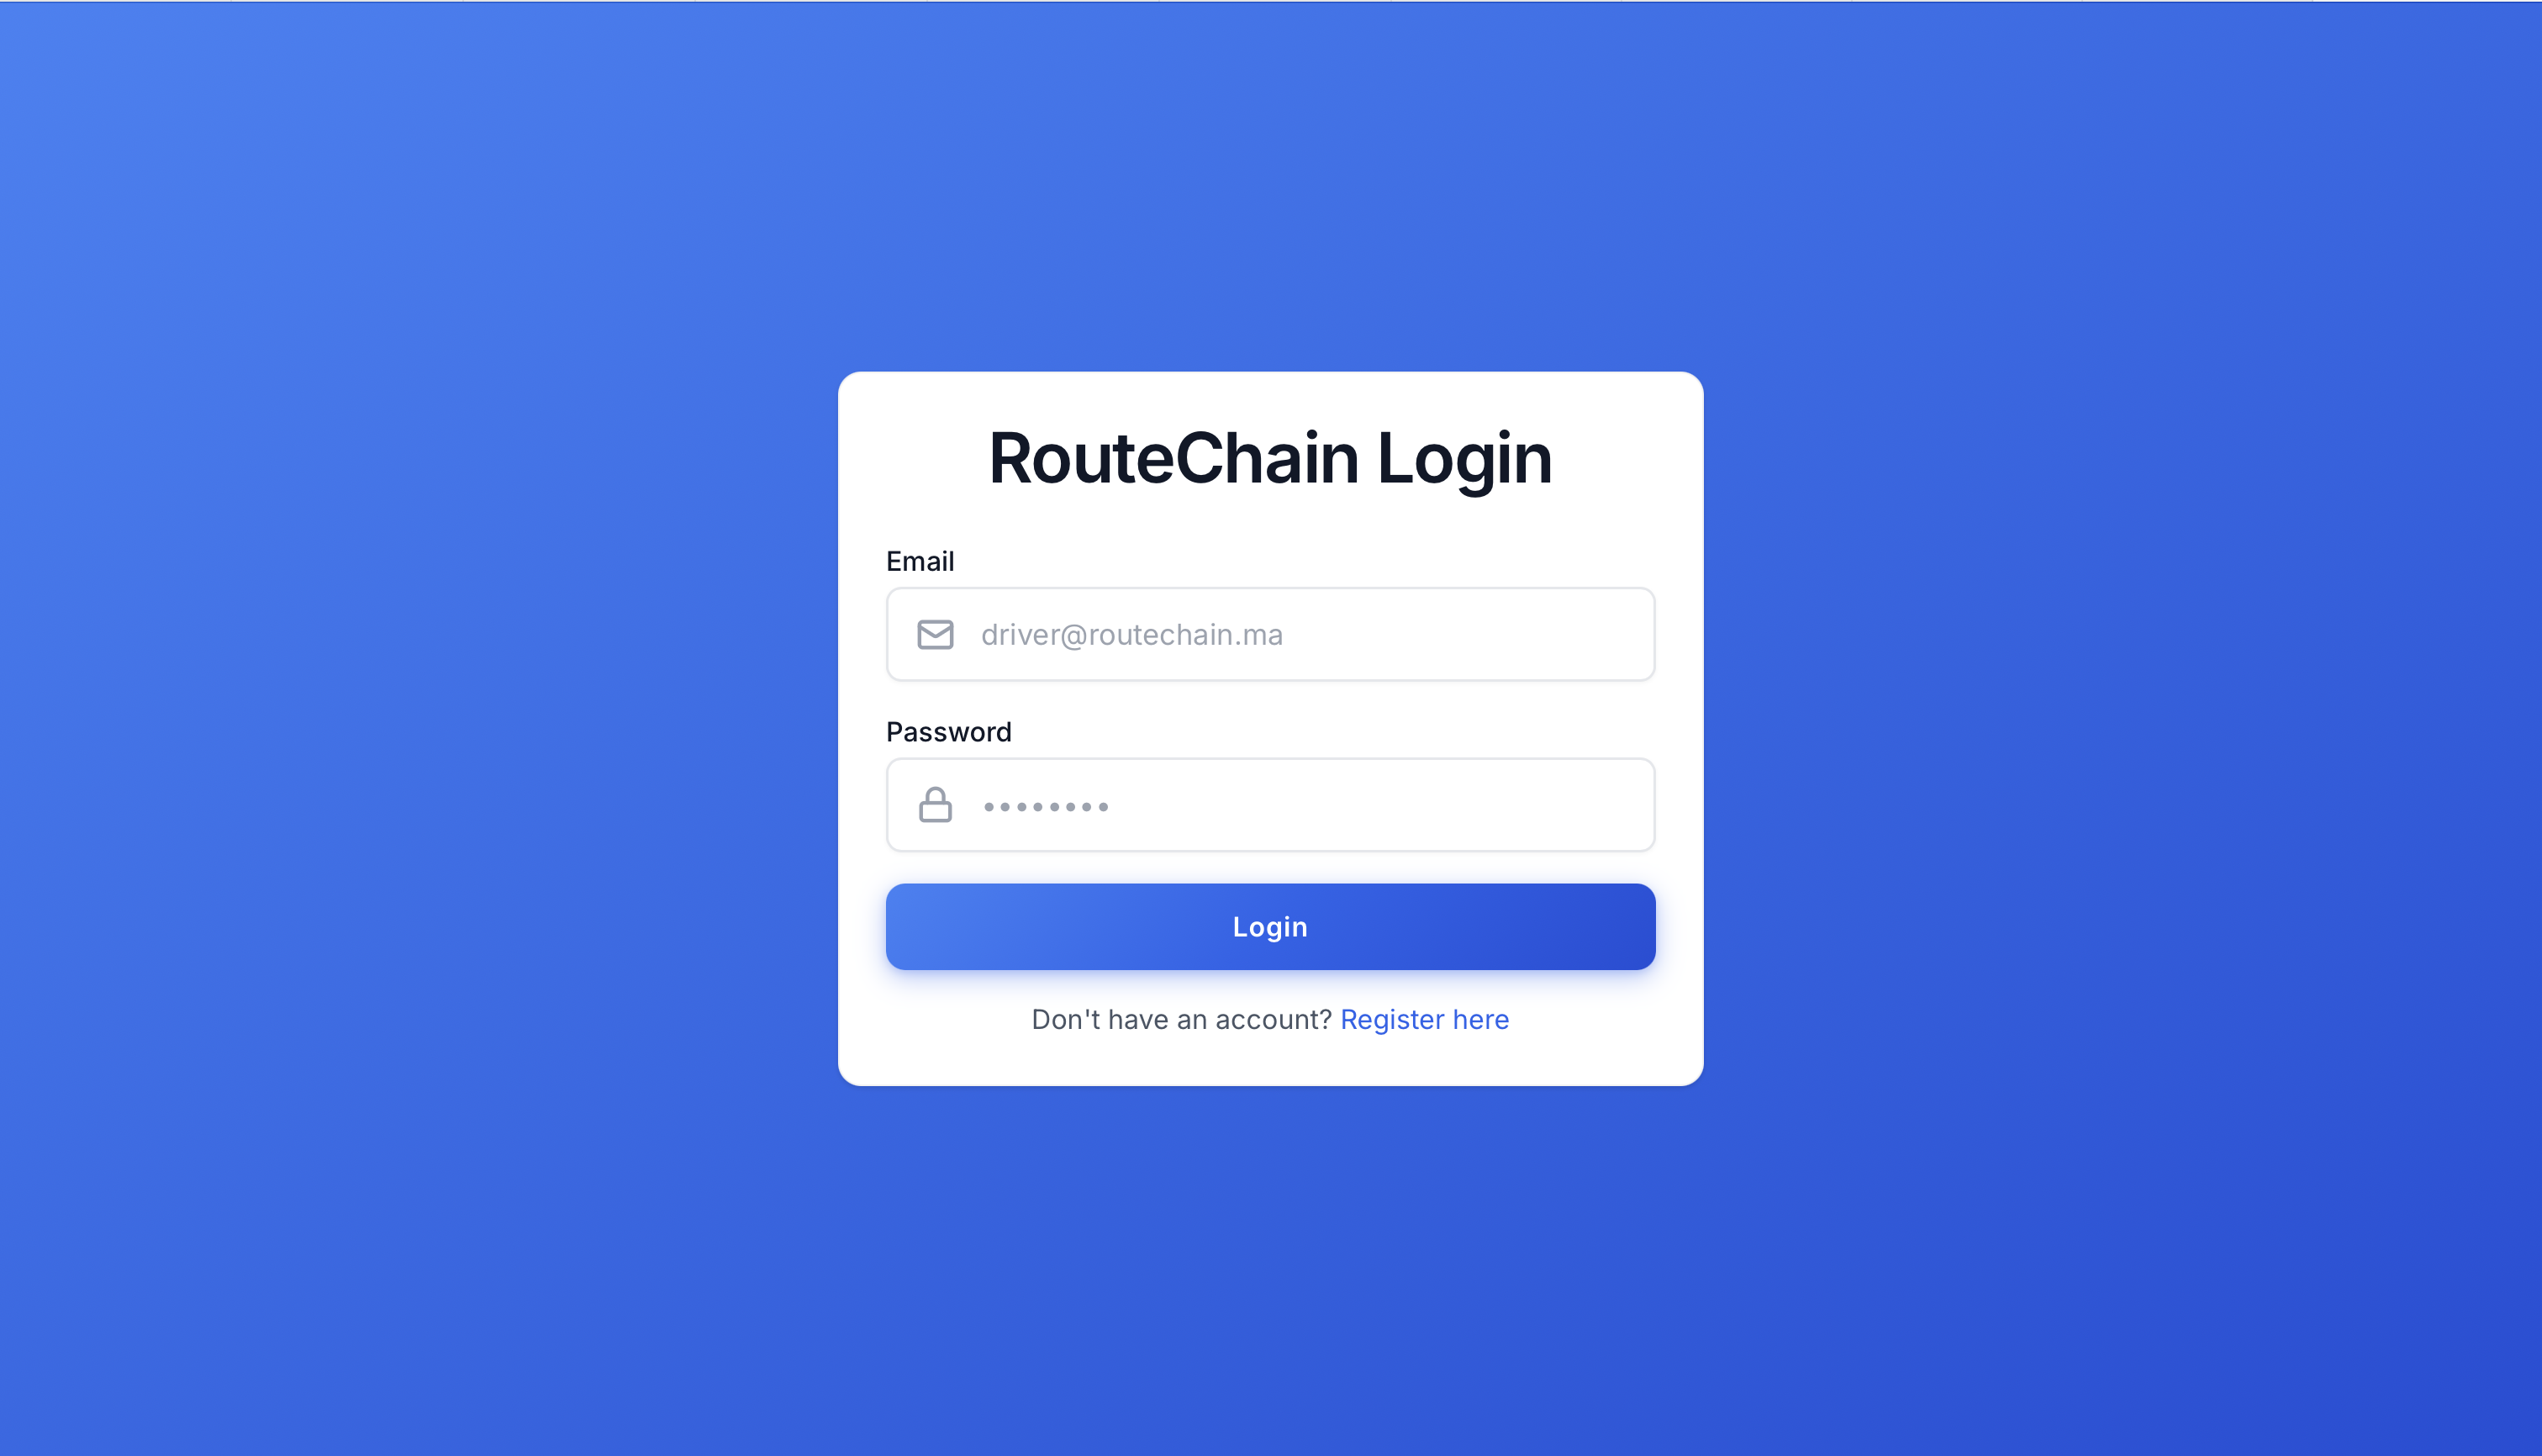
\includegraphics[width=0.92\textwidth]{resultats/login.png}
\caption{Page de connexion de l'application RouteChain}
\label{fig:screen_login}
\end{figure}

Le formulaire d'inscription permet la création d'un nouveau compte chauffeur avec validation en temps réel des champs. L'interface guide l'utilisateur à travers les informations requises : nom complet, adresse email, mot de passe avec indicateur de force, numéro de téléphone au format marocain, type de véhicule (moto, voiture, van, camion) et capacité maximale de colis. Cette conception assure que les données des chauffeurs sont complètes dès leur inscription.

\begin{figure}[H]
\centering
\includegraphics[width=0.92\textwidth]{resultats/register.png}
\caption{Page d'inscription avec formulaire de création de compte chauffeur}
\label{fig:screen_register}
\end{figure}

\subsection{Dashboard et Gestion des Tournées}

Le tableau de bord principal constitue le point d'entrée après connexion. Il affiche une vue d'ensemble des tournées du chauffeur avec des indicateurs clés : nombre de tournées actives, tournées complétées aujourd'hui, et distance totale parcourue. Chaque tournée est représentée sous forme de carte avec son nom, statut (planifiée, en cours, complétée), distance totale et nombre de points de livraison. Des boutons d'accès rapide permettent de créer une nouvelle tournée, gérer les clients et consulter les dépôts.

\begin{figure}[H]
\centering
\includegraphics[width=0.92\textwidth]{resultats/dashboard.png}
\caption{Dashboard principal affichant la liste des tournées}
\label{fig:screen_dashboard}
\end{figure}

\subsection{Création de Tournée}

L'interface de création de tournée est le cœur fonctionnel de l'application. Elle se divise en trois sections principales : les informations de la tournée (nom), la sélection du dépôt de départ, et l'ajout des points de livraison. L'utilisateur peut soit sélectionner un dépôt préexistant dans la base de données, soit saisir manuellement une adresse. Le géocodage automatique via l'API Nominatim (OpenStreetMap) convertit instantanément les adresses textuelles en coordonnées GPS précises.

\begin{figure}[H]
\centering
\includegraphics[width=0.92\textwidth]{resultats/create_route1.png}
\caption{Formulaire de création de tournée - Section dépôt et informations}
\label{fig:screen_route_form1}
\end{figure}

La section des points de livraison permet d'ajouter entre 1 et 20 destinations. Pour chaque point, l'utilisateur peut soit sélectionner un client existant (qui remplit automatiquement les coordonnées), soit saisir un nouveau client avec son nom, téléphone, adresse et instructions de livraison. Une prévisualisation cartographique interactive affiche en temps réel tous les points sur une carte Leaflet, permettant de valider visuellement les positions avant l'optimisation.

\begin{figure}[H]
\centering
\includegraphics[width=0.92\textwidth]{resultats/create_route2.png}
\caption{Formulaire de création de tournée - Points de livraison et carte}
\label{fig:screen_route_form2}
\end{figure}

\subsection{Détail de Tournée et Visualisation Cartographique}

La page de détail présente toutes les informations d'une tournée optimisée. Elle affiche la liste ordonnée des points de livraison selon l'ordre optimal calculé par Google OR-Tools, avec pour chaque point : le nom du client, l'adresse, le numéro de séquence et le statut de livraison. Les statistiques globales incluent la distance totale, le temps estimé et le nombre de colis. Des boutons d'action permettent de démarrer la tournée, confirmer les livraisons et exporter les données.

\begin{figure}[H]
\centering
\includegraphics[width=0.92\textwidth]{resultats/route_details1.png}
\caption{Page de détail d'une tournée avec informations et carte}
\label{fig:screen_route_detail1}
\end{figure}

La carte interactive affiche l'itinéraire optimisé avec des marqueurs numérotés pour chaque point de livraison. Le tracé polyline suit les routes réelles grâce à l'API OpenRouteService, offrant une visualisation précise du parcours. L'interface affiche également les informations de traçabilité blockchain : hash de transaction, numéro de bloc et horodatage d'enregistrement. Le bouton de vérification permet de contrôler l'intégrité des données en comparant le hash stocké avec celui recalculé.

\begin{figure}[H]
\centering
\includegraphics[width=0.92\textwidth]{resultats/route_details2.png}
\caption{Visualisation cartographique et informations blockchain}
\label{fig:screen_route_detail2}
\end{figure}

\subsection{Profil Utilisateur}

La page de profil permet au chauffeur de consulter et modifier ses informations personnelles. Elle affiche le nom complet, l'adresse email, le numéro de téléphone, le type de véhicule utilisé et la plaque d'immatriculation. Des statistiques de performance sont également présentées : nombre total de tournées effectuées, distance cumulée parcourue et taux de complétion. L'utilisateur peut mettre à jour ses informations via un formulaire d'édition accessible.

\begin{figure}[H]
\centering
\includegraphics[width=0.88\textwidth]{resultats/profile.png}
\caption{Page de profil du chauffeur avec informations personnelles}
\label{fig:screen_profile}
\end{figure}

\subsection{Gestion des Clients}

L'interface de gestion des clients offre une vue complète de la base de données clients. Elle présente la liste des clients enregistrés avec leurs coordonnées : nom, email, téléphone, entreprise et adresse. Une barre de recherche permet de filtrer rapidement les clients par nom ou email. Le formulaire d'ajout intègre le géocodage automatique pour convertir les adresses en coordonnées GPS, facilitant l'ajout de nouveaux clients lors de la création de tournées.

\begin{figure}[H]
\centering
\includegraphics[width=0.88\textwidth]{resultats/customers.png}
\caption{Interface de gestion des clients avec recherche et géocodage}
\label{fig:screen_customers}
\end{figure}

\subsection{Gestion des Dépôts}

La gestion des dépôts permet de définir les points de départ des tournées. L'interface affiche les dépôts enregistrés sous forme de cartes avec leur nom, adresse, coordonnées GPS et horaires d'ouverture. Un dépôt peut être marqué comme défaut pour la sélection automatique lors de la création de tournées. Le formulaire d'ajout inclut le géocodage automatique via Nominatim, permettant de convertir une adresse textuelle en latitude/longitude précises.

\begin{figure}[H]
\centering
\includegraphics[width=0.9\textwidth]{resultats/depots.png}
\caption{Interface de gestion des dépôts avec géocodage automatique}
\label{fig:screen_depots}
\end{figure}

\subsection{Panel Administrateur}

Le panel administrateur est réservé aux utilisateurs disposant du rôle admin. Il offre une vue d'ensemble de tous les chauffeurs enregistrés dans le système avec leurs informations : nom, email, type de véhicule et rôle actuel. L'administrateur peut modifier les rôles des utilisateurs (promotion en admin ou rétrogradation en driver), consulter l'historique complet des tournées de chaque chauffeur et gérer les accès au système.

\begin{figure}[H]
\centering
\includegraphics[width=0.9\textwidth]{resultats/admin_panel.png}
\caption{Panel d'administration avec gestion des chauffeurs}
\label{fig:screen_admin}
\end{figure}

\subsection{Dashboard Analytique}

Le tableau de bord analytique présente des indicateurs clés de performance (KPI) sous forme de visualisations graphiques. Il affiche le nombre total de tournées effectuées, la distance totale parcourue, le nombre de livraisons complétées et le taux de complétion moyen. Des graphiques d'évolution temporelle permettent d'analyser les tendances sur différentes périodes. Cette interface aide les gestionnaires à évaluer l'efficacité des opérations de livraison.

\begin{figure}[H]
\centering
\includegraphics[width=0.95\textwidth]{resultats/analytics_dash.png}
\caption{Tableau de bord analytique avec indicateurs de performance}
\label{fig:screen_analytics}
\end{figure}

%---------------------------------------------------------------------
\section{Conclusion}
%---------------------------------------------------------------------

Ce chapitre a présenté les technologies utilisées pour le développement de RouteChain. Chaque choix technologique a été justifié en fonction des besoins spécifiques du projet : performance pour FastAPI, flexibilité pour MongoDB, puissance d'optimisation pour OR-Tools, et traçabilité pour Ganache/Ethereum.

L'architecture modulaire et les technologies modernes sélectionnées garantissent la maintenabilité et l'évolutivité du système. Le chapitre suivant proposera une discussion sur les défis rencontrés et l'évaluation du système.

